\selectlanguage{italian}

I leptoni sono le particelle fondamentali più leggere, se comparate ai sistemi formati da quarks (mesoni e barioni); fa eccezione il tauone ($ 1.78\gev/c^2 $). Sono divisi in tre generazioni, detti anche flavours, ciascuna composta da una particella di carica elettrica $ q = -1e $ ed un neutrino elettricamente neutro; inoltre, i leptoni non sono soggeti all'interazione forte.

\section{Raggi cosmici}

I \textit{raggi cosmici} (o astroparticelle) sono particelle o gruppi di particelle ad alte energie che si muovono nello spazio a velocità relativistiche: principalmente si tratta di protoni e nuclei atomici. Essi possono avere origine solare, galattica o anche extragalattica.\\
All'impatto con l'atmosfera, i raggi cosmici producono delle \textit{showers} di patricelle secondarie a causa dell'interazione con le molecole atmosferiche: parte di queste showers riesce ad arrivare sulla superficie terrestre, risultando dunque rilevabile a terra, mentre la maggior parte viene deflessa nello spazio dalla magnetosfera.\\
Lo studio approfondito dei raggi cosmici è importante principalmente perché costituiscono una fonte di pericolo per missioni spaziali ed extraplanetarie: essi causano danni ai sistemi elettronici e biologici non protetti da un'atmosfera o una magnetosfera, dunque sono una complicazione  per missioni lunari e marziane. In maniera non secondaria, gli ultra-high-energy cosmic rays (UHECRs) possono raggiungere energie fino a $ 3\cdot10^{20}\ev $ (massimo finora osservato), di svariati ordini di grandezza superiori a quelle raggiungibili negli accelleratori odierni: si parla infatti di accelleratori cosmici.

\subsection{Osservazioni}

Le prime osservazioni di raggi cosmici furono svolte da Hess et al. nel 1912 con un pallone aerostatico: misurando la radiazione inonizzante in funzione dell'altezza, si scoprì che essa aumentava man mano che si allontanava dalla superficie terrestre. La conclusione fu che la sorgente di questa radiazione doveva essere extraplanetaria: la causa della ionizzazione dell'atmosfera sono appunto i raggi cosmici. La maggior parte della radiazione dovuta ai raggi cosmici è assorbita dall'atmosfera o deflessa nello spazio, ma una parte riesce ad arrivare alla superficie terrestre.

\subsubsection{Primary Cosmic Rays}

I raggi cosmici primari sono quelli che collidono direttamente con l'atmosfera terrestre: sono costituiti principalmente da protoni e raggi $ \alpha $ (nuclei di idrogeno ed elio), ma una frazione relativamente piccola è costituita dai cosiddetti \textit{ioni HZE} (high atomic number and energy), i quali sono nuclei di atomi pesanti ($ Z > 2 $) con cariche elettriche maggiori di $ +3e $. Quest'ultimi sono particolarmente pericolosi per i cosmonauti, poiché contribuiscono in maniera significativa alla loro dose assorbita di radiazione.\\
In Fig. \ref{flux-cr} è riportato il flusso incidente di raggi cosmici: si può vedere che l'andamento non è liscio ma presenta tre picchi, detti knees ed ankle: si pensa che i due knees siano dovuti al fatto che gli accelleratori di raggi cosmici galattici abbiamo un massimo energetico oltre il quale non possono accellerare particelle, mentre l'ankle dovrebbe corrispondere ad una zona dominata dai raggi cosmici extragalattici, sebbene ci sia ancora molta incertezza su questi dati.

\begin{figure}
	\centering
	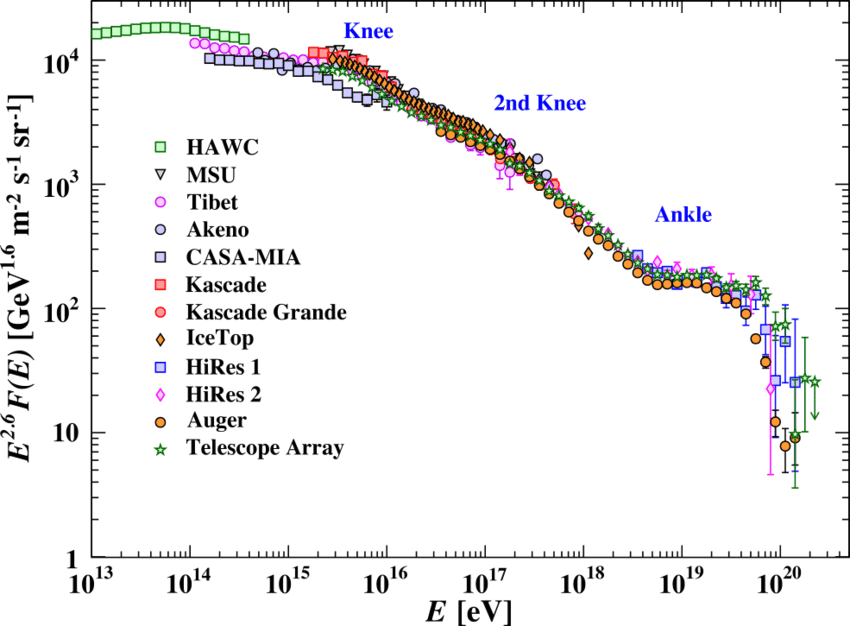
\includegraphics[width=0.70\textwidth]{cosmic-rays.png}
	\caption{Flux of cosmic rays.}
	\label{flux-cr}
\end{figure}

\subsubsection{Secondary Cosmic Rays}

Interagendo con le molecole nell'atmosfera, i raggi cosmici primari producono showers di particelle, dette raggi cosmici secondari: questi sono principalmente pioni, ma una frazione minore è composta da kaoni, protoni, neutroni e rispettive antiparticelle. La componente mesonica (pioni e kaoni) decade principalmente producendo muoni e neutrini:

\begin{equation*}
	\pi^0 \rightarrow \gamma + \gamma \qquad \pi^+ \rightarrow \mu^+ + \bar{\nu}_{\mu} \qquad \pi^- \rightarrow \mu^- + \nu_{\mu}
\end{equation*}
\begin{equation*}
	K^{\pm} \rightarrow \pi^{\pm} + \pi^0 \qquad K^+ \rightarrow \mu^+ + \bar{\nu}_{\mu} \qquad K^- \rightarrow \mu^- + \nu_{\mu}
\end{equation*}

Importanti studi sui raggi cosmici secondari sono stati svolti da Bruno Rossi: nel 1932, si accorse della presenza di due componenti nelle showers, un \textit{soft component} ed un \textit{hard component}. Il soft component, circa il 30\% della radiazione secondaria, è costituita dalle electromagnetic showers, dovute principalmente al decadimento del $ \pi^0 $ e costituite da coppie elettrone-positrone e fotoni ad alta energia: il nome è dovuto al fatto che queste particelle vengono bloccate da pochi millimetri di materiale assorbente. L'hard component, invece, costituisce il 70\% della radiazione secondaria ed è costituito dalle hadronic showers: queste comprendono principalmente muoni e, se sufficientemente energetici, possono penetrare vari metri di materiale assorbente.

\paragraph{Pierre Auger Observatory}

Il Pierre Auger Observatory è un osservatorio internazionale di raggi cosmici secondari situato in Argentina: il suo obbiettivo è la rilevazione di UHECRs con energie $ \gtrsim 10^{18}\ev $. Questi hanno un flusso stimato di $ 1\,\text{km}^{-2} / 100\,\text{y} $, dunque è necessaria una vasta area d'osservazione: essendo composto da 200 water tanks con detection area di $ 12\,\text{km}^2 $, il PAO ha una detection area complessiva di oltre $ 3000\,\text{km}^2 $, comparabile alla superficie del Lussemburgo.\\
In particolare, l'osservazione precisa delle showers da parte di numerose water tanks permette di estrapolare informazioni sulla direzione del cosmic ray e sulla posizione approssimativa della sua sorgente.

\subsection{Muoni}

Il muone è stata la prima particella fondamentale instabile scoperta: esso ha $ m_{\mu} = 105.7\mev/c^2 $, $ \tau = 2.196\,\mu\text{s} $, $ q = -1e $ e $ s = \frac{1}{2} $. Inizialmete si era pensato che fosse il mesone di Yukawa, ovvero il mediatore dell'interazione forte (all'epoca detto mesotrone), ma studiando il suo decadimento si notò che non c'erano legami tra il muone ed i nucleoni:
\begin{equation*}
	\mu^- \rightarrow e^- + \bar{\nu}_e + \nu_{\mu}
\end{equation*}
Questo è un esempio di conservazione del numero leptonico: a ciascuna famiglia leptonica è associato un numero leptonico, il quale deve essere conservato nei decadimenti: ai leptoni è associato $ +1 $, mentre agli antileptoni $ -1 $, dunque nel decadimento del muone devono rimanere costanti $ L_e = 0 $ ed $ L_{\mu} = +1 $, ergo la presenza di $ \bar{\nu}_e $ e $ \nu_{\mu} $.\\
Il muone costituisce anche un perfetto esempio di cinematica relativistica: assumendo che vengano prodotti muoni a $ 10\,\text{km} $ dalla superficie terrestre a causa di raggi cosmici e che essi si muovano a velocità $ 0.98c $, essi impiegherebbero $ t = 34\,\mu\text{s} $ per arrivare a terra; data la vita media del muone $ t_{1/2} = 1.56\,\mu\text{s} $, a terra dovrebbe giungere una frazione del flusso iniziale pari a $ 2^{-34/1.56} = 0.27\cdot10^{-6} $, praticamente nulla. Non si sta però contando la dilatazione relativistica dei tempi: per il muone $ \gamma \approx 5 $, dunque la vita media nel suo rest-frame è sempre $ 1.56\,\mu\text{s} $, ma per un osservatore a riposo rispetto alla Terra essa è $ t'_{1/2} = \gamma t_{1/2} = 7.8\,\mu\text{s} $: la frazione di flusso osservata nel frame della Terra è quindi $ 0.049 $, che è quella effettivamente misurata. Alternativamente, si può anche svolgere il calcolo nel rest-frame dei muoni, considerando dunque la contrazione delle lunghezze: nel loro frame, i muoni non percorrono $ 10\,\text{km} $, bensì $ 2\,\text{km} $.\\
I muoni costituiscono la principale fonte di rumore nella misura degli eventi rari a terra, con un flusso medio al livello del mare di $ 1\,\text{cm}^{-2} / \text{min} $: una soluzione per l'eliminazione del muon background è quella di costruire laboratori sotterranei, specialmente sotto montagne rocciose alte (es.: il Gran Sasso).

\paragraph{Scoperta}

Nel 1936 Anderson e Neddermeyer, studiando la radiazione cosmica al Caltech, si accorsero di particelle che, in presenza di un campo magnetico, curvavano in maniera simile agli elettroni ma con raggio diverso: in particolare, la curva era più larga di quella degli elettroni, ma più stretta di quella dei protoni, dunque si evinse l'esistenza di una particella simile all'elettrone ma con massa intermedia tra quella dell'elettrone e quella del fotone.\\
Per quanto riguarda invece la misura della vita media del muone, il principale limite è posto dagli effetti relativistici che entrano in gioco per i muoni cosmici. per questo motivo, Rasetti e Rossi usarono il coincidence method ideato da Bothe: un circuito elettronico integrato in uno scintillatore di grosse dimensioni segna il tempo di arrivo del muone in esso ed il tempo in cui avviene il suo decadimento (emissione di elettrone o positrone). Con un circuito sufficientemente raffinato, si riuscì a misurare la vita media del muone.

\paragraph{Tauone}

Oltre all'elettrone ed al muone, la terza famiglia leptonica è quella del tauone e del neutrino tauonico: il primo fu inizialmente teorizzato da Yung-su Tsai nel 1971 e successivamente osservato da Perl nel 1974, mentre il secondo fu osservato solo nei primi anni 2000. Un tentativo italiano di rilevare il tauone fu fatto da Zichichi negli anni '60 col collisore di elettroni e positroni ADONE a Frascati, la le energie raggiunte non erano sufficienti per la reazione $ e^- + e^+ \rightarrow \tau^- + \tau^+ $.\\
Il tauone è analogo all'elettrone ed al muone, con una massa molto più alta $ m_{\tau} = 1.777\gev/c^2 $. I suoi principali decay branches sono:
\begin{equation*}
	\tau^- \rightarrow e^- + \bar{\nu}_e + \nu_{\tau}
	\qquad
	\tau^- \rightarrow \mu^- + \bar{\nu}_{\mu} + \nu_{\tau}
\end{equation*}

\section{Neutrini}

Essendo elettricamente neutri, i neutrini interagiscono solo tramite interazione debole: dato che la loro interaction cross-section è praticamente nulla, non si riesce ad osservarli direttamente con rilevatori e le loro proprietà vanno inferite in maniera indiretta.\\
Le prime evidenze indirette dell'esistenza dei neutrini si ebbero con lo studio del decadimento $ \beta $: per spiegare l'apparente violazione della conservazione dell'energia, Pauli postulò che esso fosse un decadimento a tre corpi, dove la terza particella era estremamente difficile da osservare. Con il successivo sviluppo della teoria di Fermi del decadimento $ \beta $ è stato possibile iniziare a stimare i parametri dei neutrini, in particolare del neutrino elettronico: dallo studio dei Fermi-Kurie plots e notando che l'energia osservata dell'elettrone prodotto dal decadimento è vincolata da $ m_e \le E_e \le \Delta M - m_{\nu_e} $, si può porre un porre dei limiti per i valori di $ m_{\nu_e} $. Ad oggi, la stima migliore è data dall'analisi del decadimento del trizio $ \ch{^3H} \rightarrow \ch{^3He} + e^- + \bar{\nu}_e $: $ m_{\nu_e} \le 0.8\ev/c^2 $.

\subsection{Neutrino detection}

Solitamente si misura l'interazione di una particella in un mezzo con dei rilevatori che identificano il segnale prodotto dall'interazione, il quale dipende dalla natura della particella: ad esempio, particelle cariche portano ad una ionizzazione del mezzo, creando coppie elettrone-ione, dunque un rilevatore potrebbe misurare la corrente elettrica prodotta; i fotoni interagiscono per effetto Compton oppure con pair production; i neutroni danno luogo a reazioni nucleari nel mezzo che inducono la produzione di particelle cariche.\\
I neutrini, però, interagiscono troppo debolmente con la materia e danno luogo a segnali troppo deboli: un neutrino necessita di $ \sim 10^{13}\,\text{km} $ (un anno luce) di piombo per essere stoppato con una probabilità del 50\%, e anche con un rilevatore grande come la Terra soltanto un neutrino su 100 miliardi interagirebbe. Lo studio dei neutrini è altresì molto importante, poiché sono particelle onnipresenti nell'Universo: la densità media di neutrini è $ \sim 10^8 \,\text{m}^{-3} $ (relic neutrinos), dunque giocano un ruolo cruciale in numerosi processi astrofisici.\\
I principali processi che producono neutrini sono di due tipi:
\begin{enumerate}
	\item reazioni nucleari a bassa energia: fusione nucleare nel Sole (sotto $ 100\kev $ per nucleone) e fissione nucleare nei reattori (neutroni termici che decadono $ \beta^- $ in $ \tau \approx 15\,\text{min} $);
	\item collisioni ad alta energia: collisori di particelle e cosmic ray showers (pioni che decadono in muoni e neutrini).
\end{enumerate}
La conferma sperimentale dell'esistenza dei neutrini è stata ottenuta nel 1956 da Cowan e Reines con un detector presso una centrale nucleare in South Carolina, la quale produce un flusso di neutrini di $ \sim 10^{19} \,\text{s}^{-1} $ (flusso effettivo nel rilevatore $ 5\cdot10^{13}\,\text{cm}^{-2}\text{s}^{-1} $). In particolare, sfruttarono la reazione del decadimento $ \beta $ inverso:
\begin{equation*}
	\bar{\nu}_e + p \rightarrow n + e^+
\end{equation*}
L'antineutrino proveniente dalla centrale inizialmente converte un protone in un neutrone, producendo un positrone: quest'ultimo si annichila con gli elettroni atomici presenti nel mezzo, generando due fotoni energetici che, per effetto Compton, generano fotoni rilevabili dal detector; mentre ciò avviene in maniera praticamente istantanea, con un delay di $ \sim 1\,\text{ms} $ il neutrone viene catturato da un atomo di $ \ch{^{113}Cd} $ nel mezzo, producendo altri fotoni. In questo modo, fu possibile misurare la sezione d'urto d'interazione degli antineutrini elettronici: $ 6.3\cdot10^{-44} \,\text{cm}^2 $, in perfetto accordo col valore teorico.\\
A seguito della scoperta del muone, si teorizzò l'esistenza del neutrino muonico, il quale fu effettivamente osservato nel 1962 da Lederman, Schwartz e Steinberger con un apparato che, producendo muoni a partire da un fascio protonico (tramite pioni e kaoni), è in grado di rilevare direttamente neutrini muonici. In maniera analoga si procedette alla teorizzazione e scoperta del neutrino tauonico.

\subsection{Neutrini solari}

Le reazioni di fusione nucleare nel Sole producono neutrini. In particolare, ci sono due principali cicli di reazioni che producono energia nel Sole (Fig. \ref{sol-cyc}): il ciclo pp ed il ciclo CNO.

\begin{figure}[!b]
	\centering
	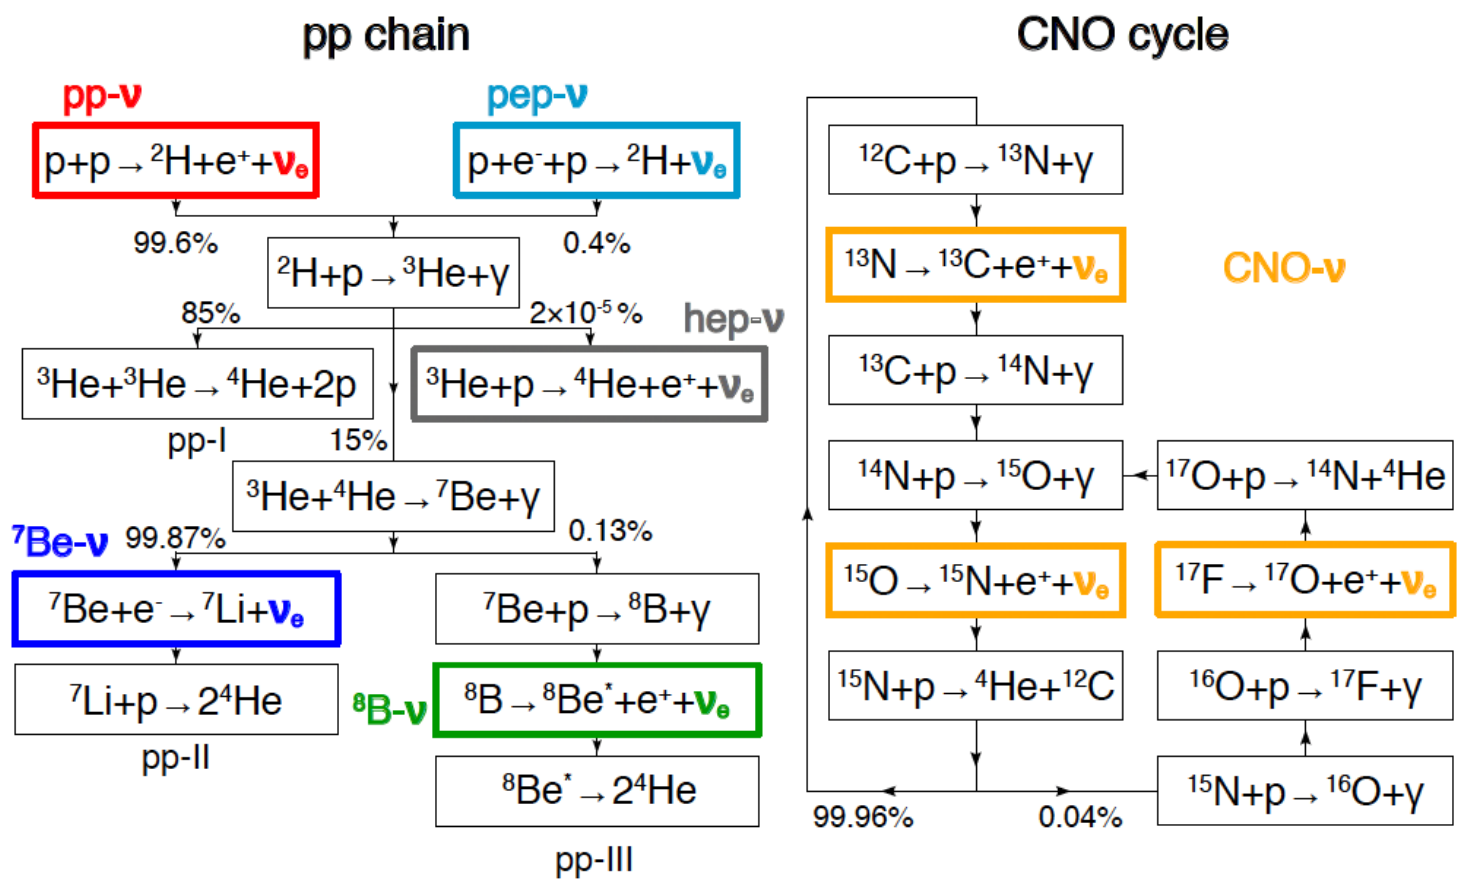
\includegraphics[width=0.70\textwidth]{solar-cycles.png}
	\caption{Nuclear fusion in the Sun via pp-cycle and CNO-cycle: neutrino production highlighted.}
	\label{sol-cyc}
\end{figure}

Il \textit{ciclo pp} costituisce la sorgente di circa il 99\% dell'output energetico solare: esso è costituito da una serie di reazioni di fusione nucleare e decadimenti deboli. Il ciclo pp è dominato dal ciclo pp-I, il quale ha un bilancio netto di reazione dato da:
\begin{equation*}
	6p \rightarrow \ch{^4He} + 2p + 2e^+ + 2\nu_e + 2\gamma + 24.68\mev
\end{equation*}
Il restante 1\% dell'output solare proviene dal \textit{ciclo CNO}, anch'esso costituito da reazioni di fusione nucleare e decadimenti deboli. Il ciclo CNO è dominato dal ciclo CNO-I, con bilancio netto:
\begin{equation*}
	\ch{^{12}C} + 4p \rightarrow \ch{^4He} + \ch{^{12}C} + 2e^+ + 2\nu_e + 3\gamma + 26.73\mev
\end{equation*}
Si vede dunque che, in entrambi i cicli, data la presenza di decadimenti deboli c'è anche produzione di neutrini elettronici: con la misura del flusso di neutrini solari si possono dunque sondare direttamente le reazioni che avvengono nel nucleo del Sole\footnote{Si ricordi che le emissioni solari rilevate direttamente provengono dalla fotosfera, non dal nucleo.}.\\
Essendo l'energia totale emessa dal Sole facilmente misurabile, è possibile stimare con precisione il flusso di neutrini solari emessi e quello incidente sulla Terra: esso è $ \approx 66\cdot10^9 \,\text{cm}^{-2}\text{s}^{-1} $. Di questi, circa il 99\% è prodotto dal ciclo pp, ma, a seconda dell'energia, i vari canali di reazione producono neutrini con sezioni d'urto diverse: in Fig. \ref{s-n-en-sp} sono riportati gli spettri energetici dei vari canali di neutrino production, mentre in Fig. \ref{s-n-fl} è riportato il flusso di neutrini solari misurato dall'esperimento Borexino ai LNGS.

\begin{figure}
	\centering
	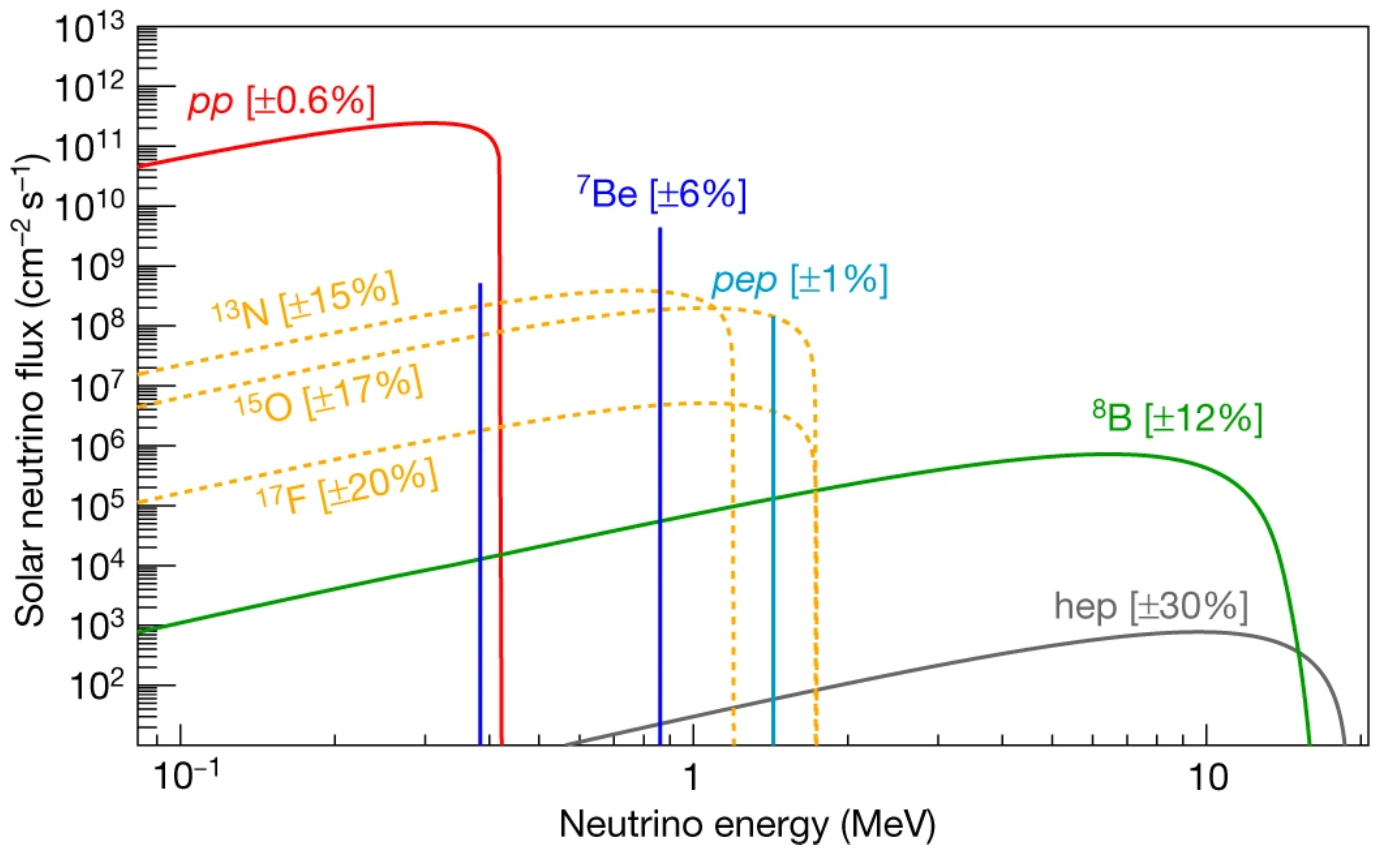
\includegraphics[width=0.70\textwidth]{sol-neutrino-en-sp.png}
	\caption{Solar neutrino energy spectra.}
	\label{s-n-en-sp}
\end{figure}
\begin{figure}
	\centering
	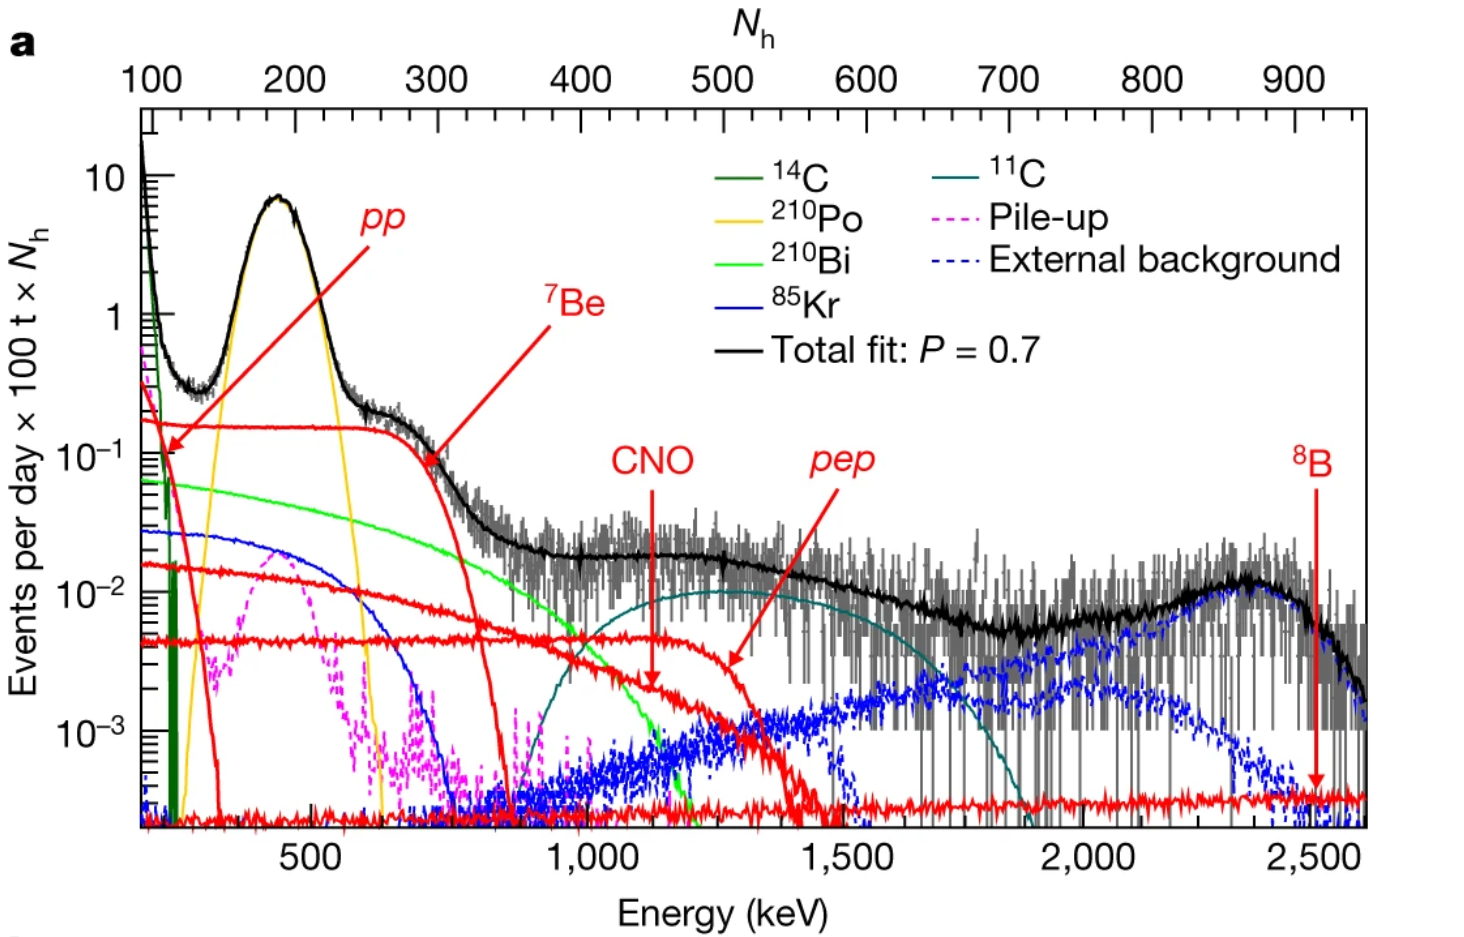
\includegraphics[width=0.70\textwidth]{sol-neutrino-flux.png}
	\caption{Solar neutrino flux measured by Borexino.}
	\label{s-n-fl}
\end{figure}

Si vede che, all'aumentare dell'energia, i canali di neutrino production hanno sezioni d'urto via via più basse: ciò determina una certa difficoltà, poiché misurare neutrini a basse energie è complicato, essendo necessario un background bassissimo. Ciò è stato l'obbiettivo dell'esperimento Borexino, situato presso i Laboratori Nazionali del Gran Sasso proprio per avere un setup il più radiopuro possibile: l'apparato consisteva in uno scintillatore sferico di notevoli dimensioni, per aumentare la probabilità d'interazione dei neutrini col liquido scintillante, contornata da fototubi per la rilevazione della radiazione Čerenkov\footnote{Emissione di luce in forma conica dovuta al fatto che la velocità della sorgente è maggiore di quella della luce nel mezzo, analogamente al moto supersonico.} prodotta dalle interazioni dei neutrini.\\
Storicamente, le prime misurazioni di neutrini solari furono svolte dal Homestake Solar Neutrino Observatory (HNSO), in South Dakota: questo era costituito da un enorme barilotto di 600 tonnellate di tetracloroetilene $ \ch{Cl_2 C = C Cl_2} $ volto alla misurazione del flusso di neutrini elettronici solari tramite il decadimento $ \beta $ inverso, secondo la reazione:
\begin{equation*}
	\nu_e + \ch{^{37}Cl} \rightarrow \ch{^{37}Ar} + e^-
\end{equation*}
Dalla misura radiometrica dell'argon fu possibile determinare che il flusso di neutrini solari era 1/3 di quello calcolato teoricamente. Questo risultato fu confermato dai rilevatori Kamiokande e SuperKamiokande in Giappone: quest'ultimo è il più grande rilevatore Čerenkov al mondo, costituito da uno scintillatore sferico di 50'000 tonnellate di acqua pura e 13'000 fotomoltiplicatori (PMTs); in particolare, la radiazione Čerenkov è emessa sia quando un neutrino interagisce con un elettrone atomico, facendolo fuoriuscire dal suo atomo, sia quando invece interagisce con un nucleone, producendo un leptone relativistico: il passaggio di queste particelle a velocità relativistiche in acqua causa l'effetto Čerenkov, il quale permette di risalire con sufficiente accuratezza alla direzione d'incidenza del neutrino.

\subsubsection{Neutrino oscillations}

Il problema dei neutrini solari rilevato dal HSNO può essere risolto supponendo che un neutrino elettronico prodotto dalle reazioni nel Sole non mantenga la sua identità lungo il tragitto fino alla Terra, ma oscilli tra le tre famiglie leptoniche: così facendo, il flusso di neutrini elettronici incidente sulla Terra sarà minore di quello previsto in precedenza. La teoria delle neutrino oscillations fu inizialmente sviluppata da Pontecorvo e poi espansa da Maki, Nakagawa e Sakata: in particolare, le neutrino oscillations sono possibili soltanto se si ammette che essi abbiano massa.\\
Si suppone che gli stati osservabili dei neutrini (elettronico, muonico, tauonico) non siano gli stessi nei quali si trovano i neutrini mentre viaggiano nello spazio: si parla di flavour eigenstates $ \ket{\nu_\alpha} $ e mass eigenstates $ \ket{\nu_j} $, legati tra loro dalla matrice PMNS:
\begin{equation}
	\ket{\nu_{\alpha}} = \sum_{j = 1}^3 U_{\alpha j} \ket{\nu_j}
	\label{eq:8.1}
\end{equation}
dove $ \alpha $ indica la famiglia leptonica ed $ j $ il mass eigenstate. L'evoluzione temporale di un mass eigenstate con energia $ E_{\nu} $, espressa in funzione della distanza $ s $ percorsa, è data da:
\begin{equation}
	\ket{\nu_j(s)} = e^{-i \frac{m_j^2}{2E_{\nu}} s} \ket{\nu_j(0)}
	\label{eq:8.2}
\end{equation}
Mass eigenstates diversi acquisteranno dunque fattori di fase diversi. Dato che, dall'Eq. \ref{eq:8.1}, i flavour eigenstates sono sovrapposizioni di mass eigenstates, un neutrino emesso con una certa identità leptonica muovendosi nello spazio avrà probabillità diverse ed oscillanti di essere rilevato con altre identità leptoniche: un esempio di oscillazioni risultanti è riportato in Fig. \ref{neutrino-oscillations}.

\begin{figure}
	\centering
	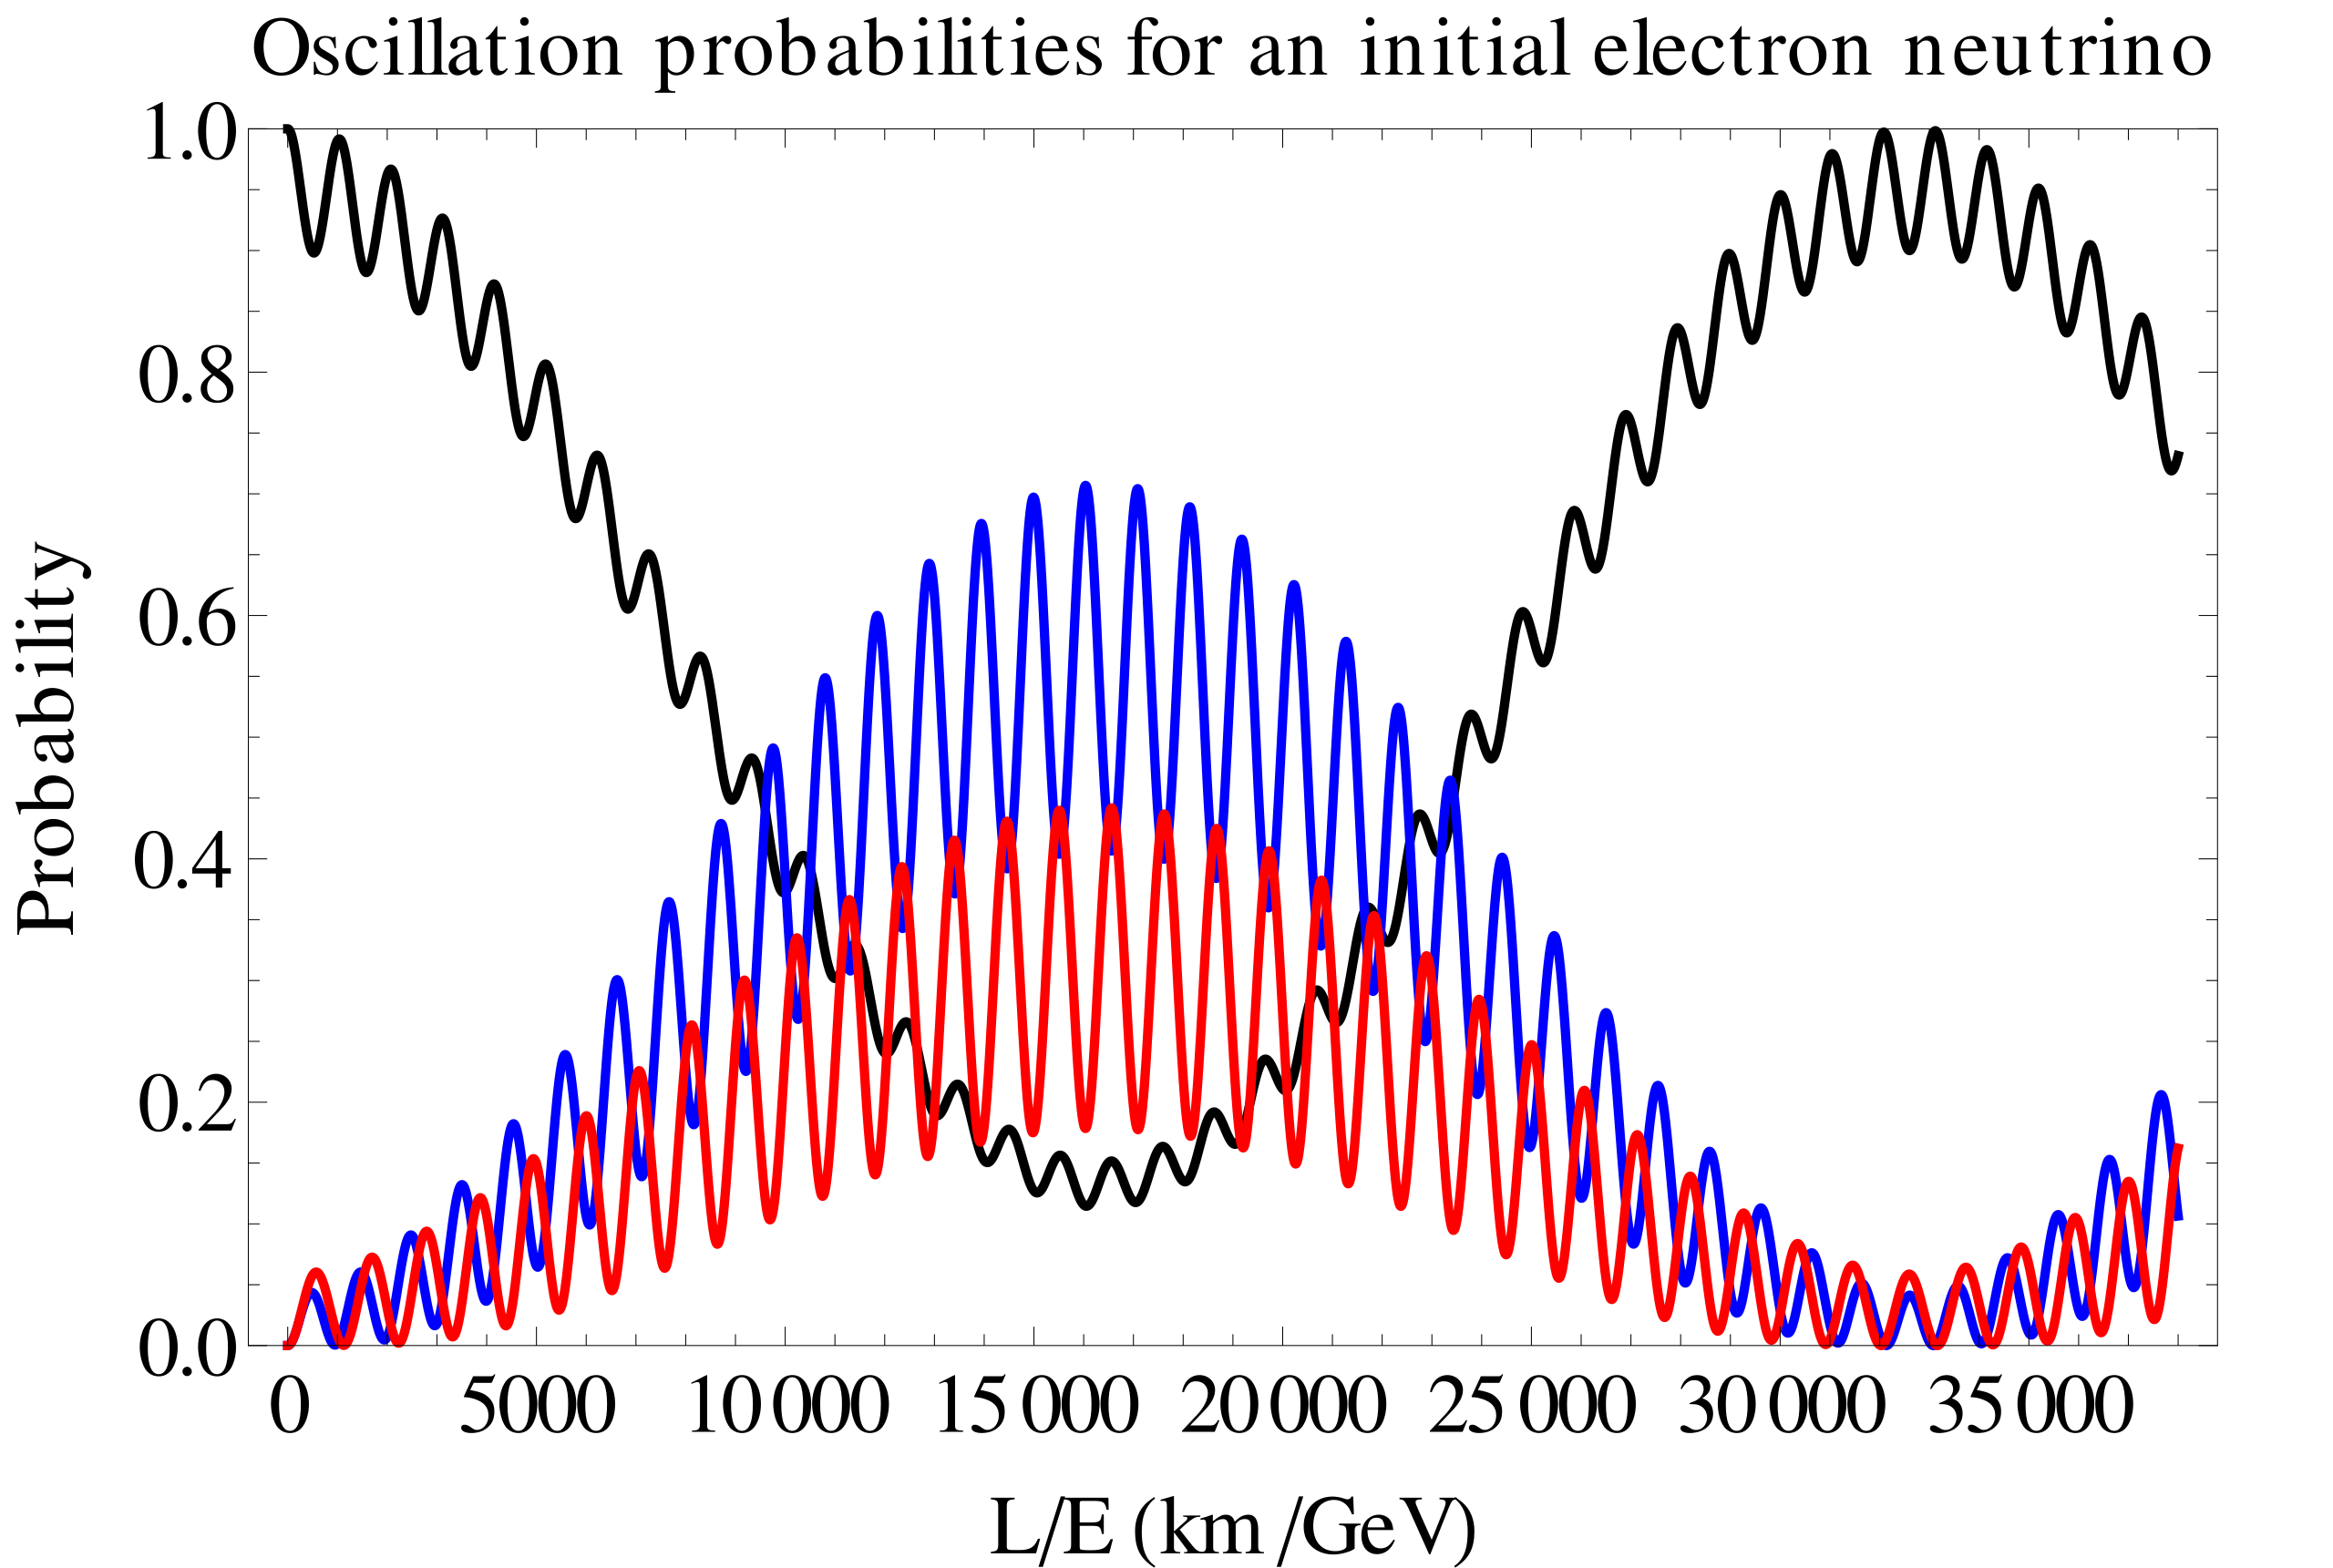
\includegraphics[width=0.60\textwidth]{neutrino-electron.png}
	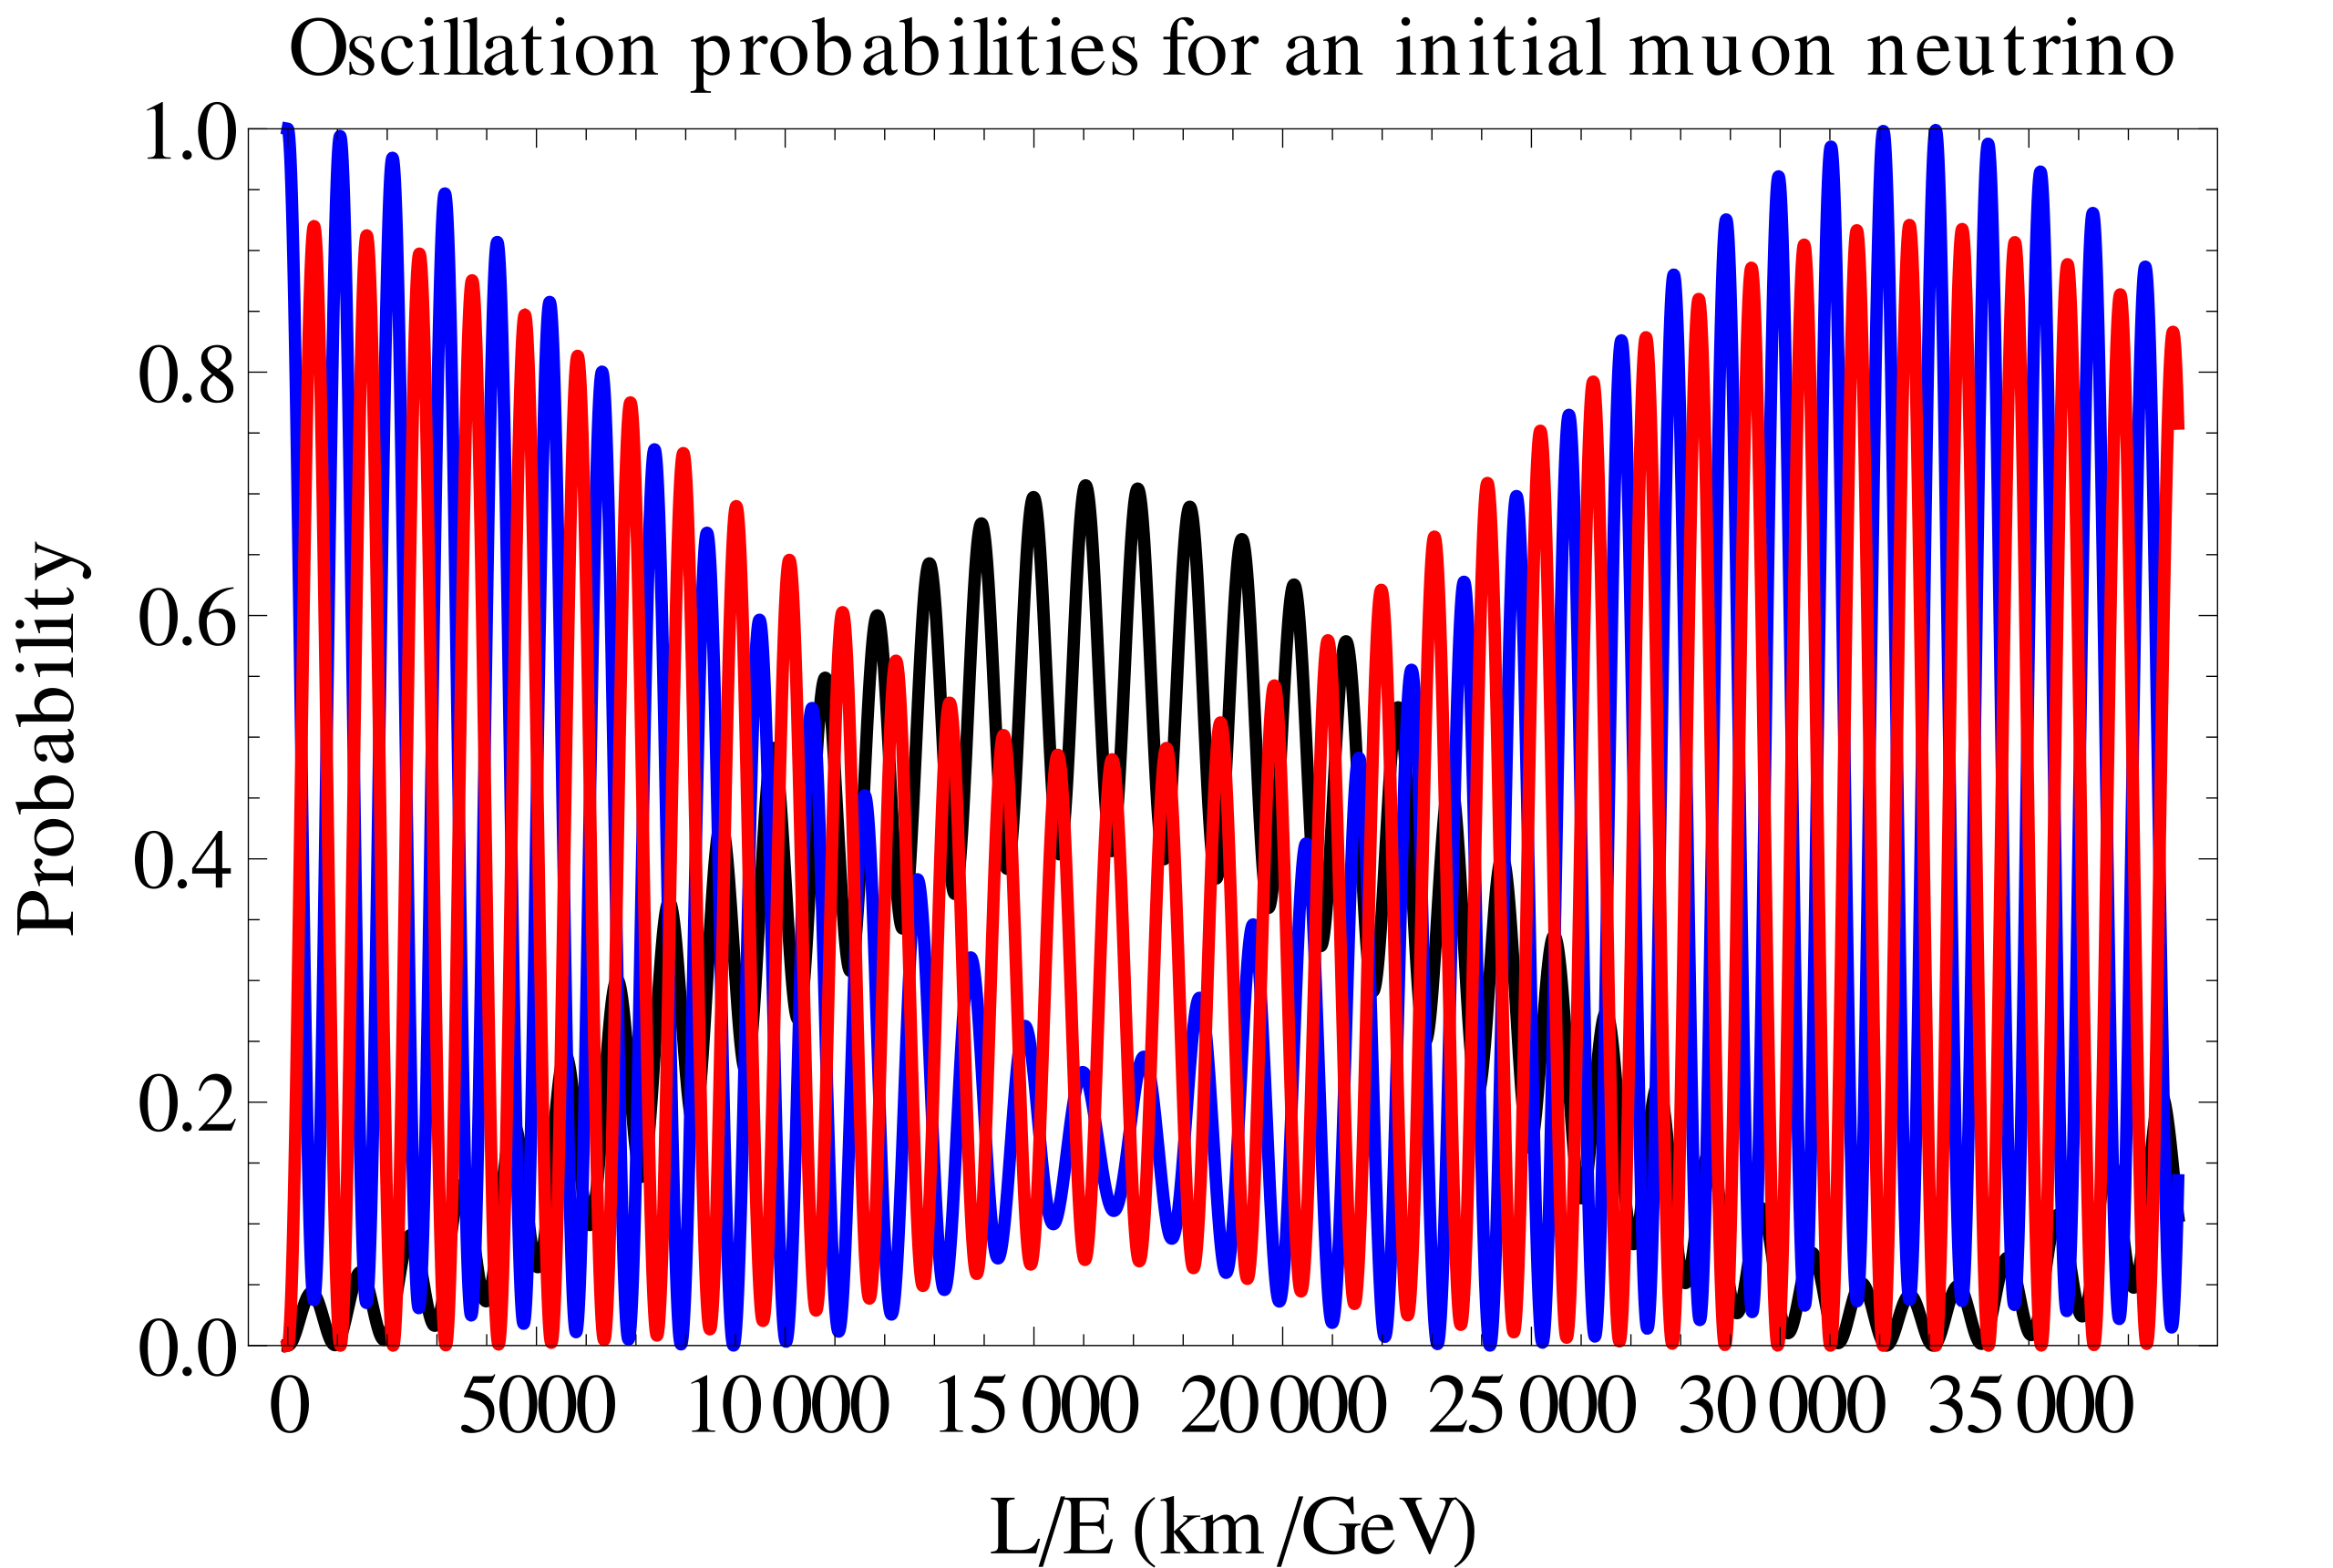
\includegraphics[width=0.60\textwidth]{neutrino-muon.png}
	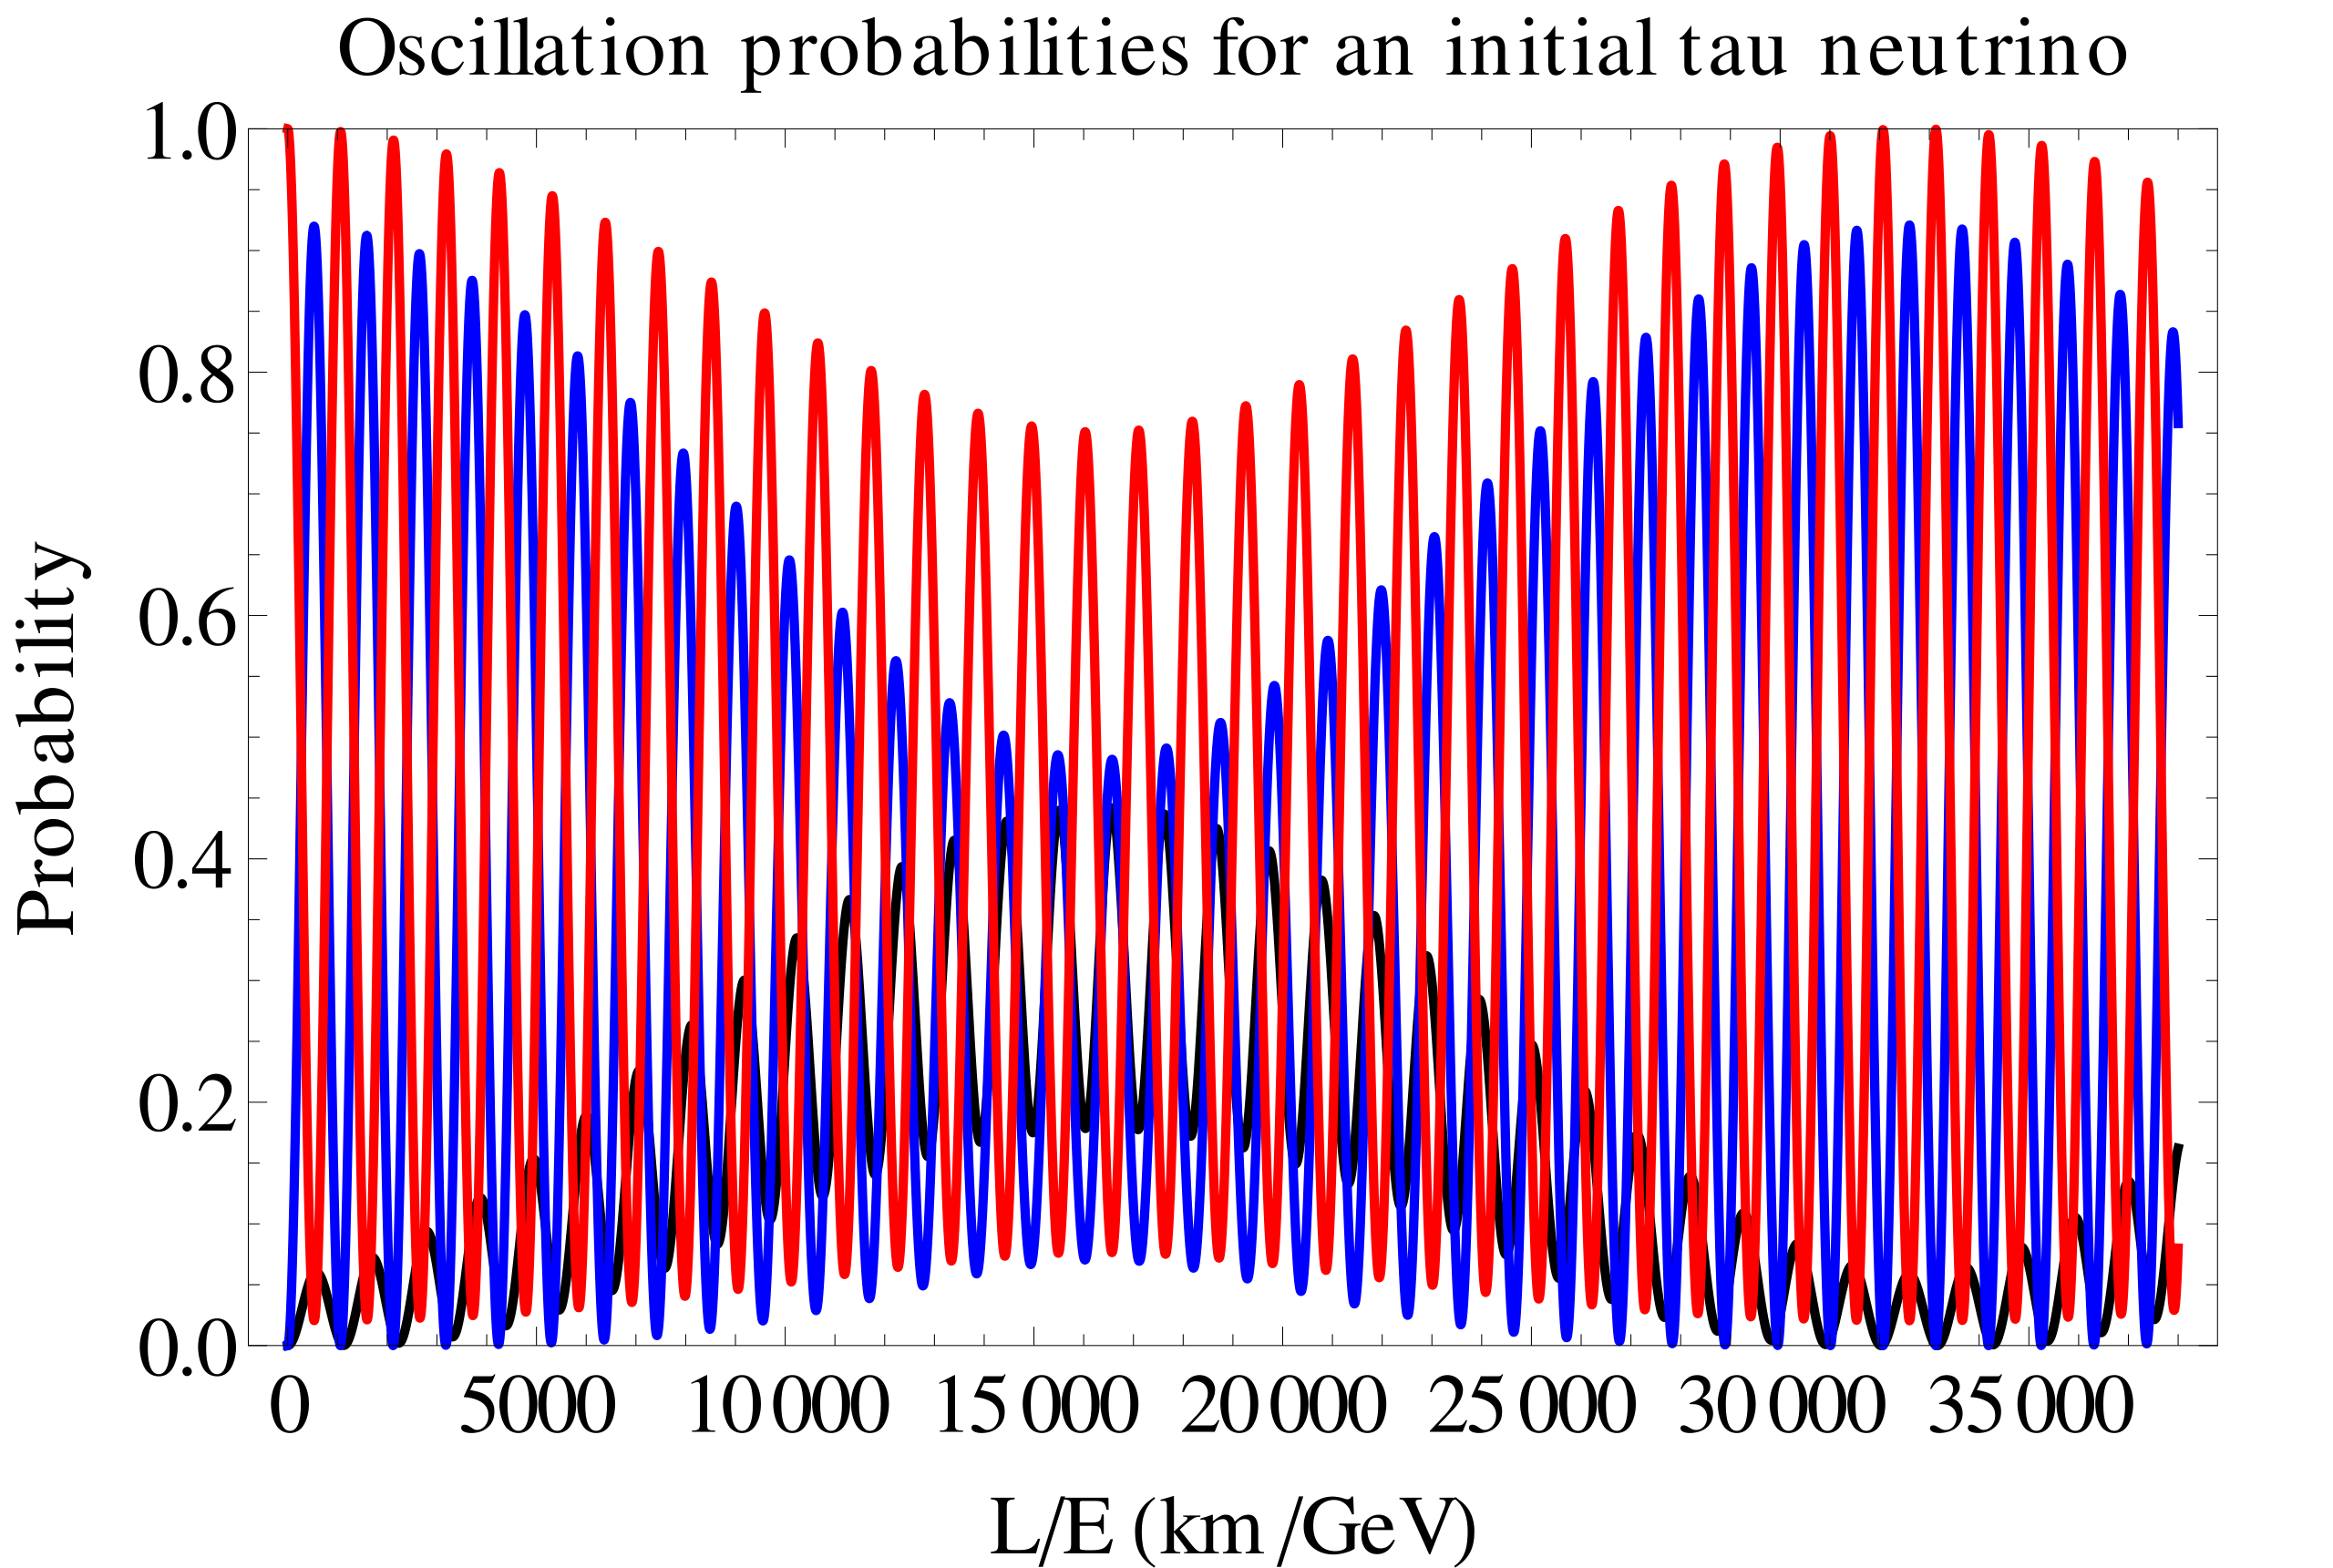
\includegraphics[width=0.60\textwidth]{neutrino-tau.png}
	\caption{Neutrino oscillations: $ \nu_e $ in black, $ \nu_{\mu} $ in blue, $ \nu_{\tau} $ in red.}
	\label{neutrino-oscillations}
\end{figure}

L'esistenza delle neutrino oscillations è stata confermata da SuperKamiokande e dal Sudbury Neutrino Observatory (SNO), valendo il Nobel del 2015 a Takaaki Kajita e Arthur Bruce McDonald. Il SNO, locato in Canada, è stato uno scintillatore sferico a base di acqua pesante (deuterio), la quale è sensibile a tutti e tre i flavours, focalizzatosi principalmente sul canale $ \ch{^8B} $ di neutrino production.\\
Il principale obbiettivo della fisica dei neutrini al momento è la misura del mass ordering: a tal fine, sono programmati gli esperimenti DUNE (USA) e JUNO (Cina). Per quanto riguarda la neutrino-based astronomy, è attivo l'IceCube Telescope in Antartide, mentre nel Mar Mediterraneo è in costruzione il KM3NeT/ORCA Telescope. Un'altra linea di ricerca è quella sull'esistenza di un eventuale quarto neutrino sterile, sebbene l'esperimento STEREO a Grenoble abbia escluso questa ipotesi.










